
\section{Static Analysis of Energy Consumption}\label{sec:energy-analysis}

Static analysis is the other key component of energy transparency.
Given an energy model assigning energy costs to some basic units of the program,
the task of analysis is to determine the overall energy consumption of the program, or
the distribution of energy consumption over the parts of the program.
Static analysis infers information about energy consumed by programs without
actually running them, in contrast to dynamic analysis, which collects information
about the program's behaviour while executing it.  Here we consider only static analysis.

As with energy modelling, analysis can be performed on
program representations at different levels 
in the software stack, ranging from source code (in different programming
languages) through intermediate compiler representations down to ISA level, and employing
an appropriate energy model at that level.



\begin{figure}
  \begin{subfigure}[b]{.49\linewidth}
  \centering
         \begin{lstlisting}
    1: void f(int n) {
          z = 1;
    2:    while (n > 0) {
             z = z*n;
             n = n-1;
    3:    }
          print(z);	
    4: }		
              \end{lstlisting}
    \caption{}
  \end{subfigure}
  \hspace{0.5cm}
  \begin{subfigure}[b]{.49\linewidth}
\begin{center}
\[
     \begin{array}{l}
	true \rightarrow r_1(n)\\
	(r_1(n) \wedge z=1)  \rightarrow r_2(n,z)\\
        (r_2(n,z)~ \wedge \\
	n < 0 \wedge z'=z*n  \wedge n'=n-1)\\
         \ \ \       \rightarrow r_3(n',z')\\
        (r_3(n',z') \wedge n=n' \wedge z=z')\\
        \ \ \         \rightarrow r_2(n,z)\\
        (r_2(n,z) \wedge n \ge 0 \wedge print(z))\\
         \ \ \      \rightarrow r_4	
     \end{array}
\]
    \end{center}
    \caption{}
  \end{subfigure}\\ \\
    \begin{subfigure}[b]{\linewidth}
\begin{center}
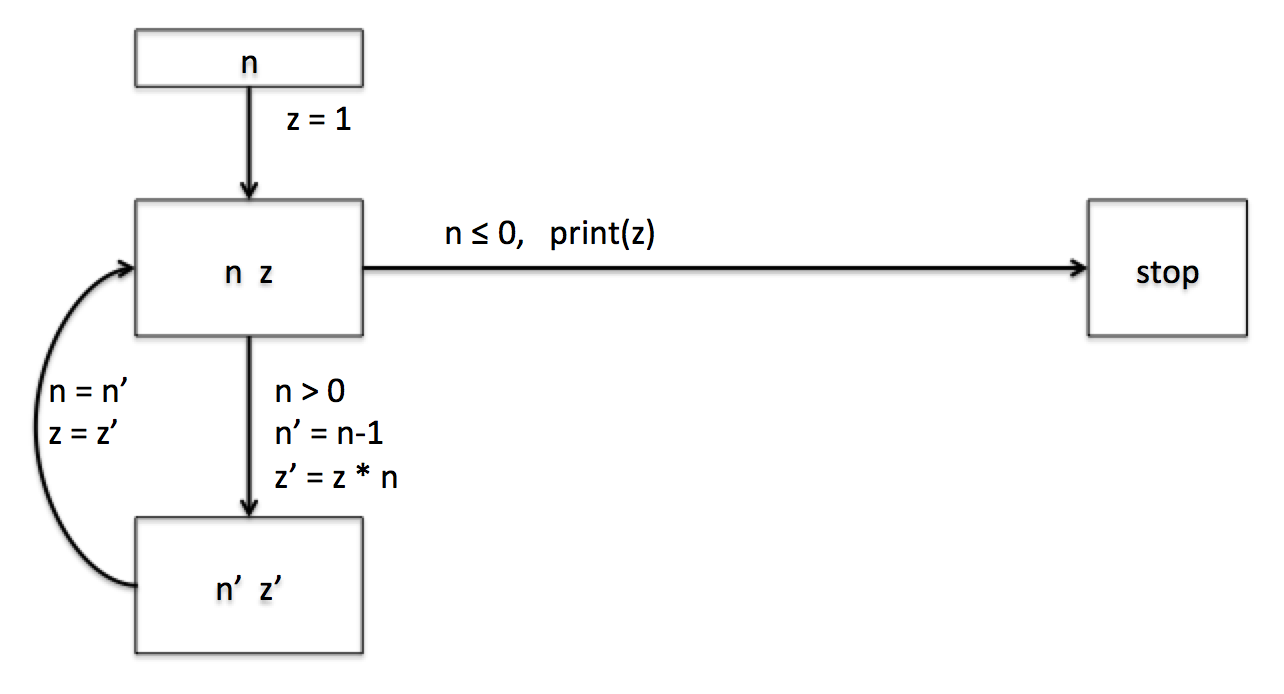
\includegraphics[width=7cm]{\figpath/transition-system}
    \end{center}
    \caption{}
  \end{subfigure}\\

  \caption{Transition system and constrained Horn clauses representing a program}
  \label{fig-horn}
\end{figure}

\begin{figure}
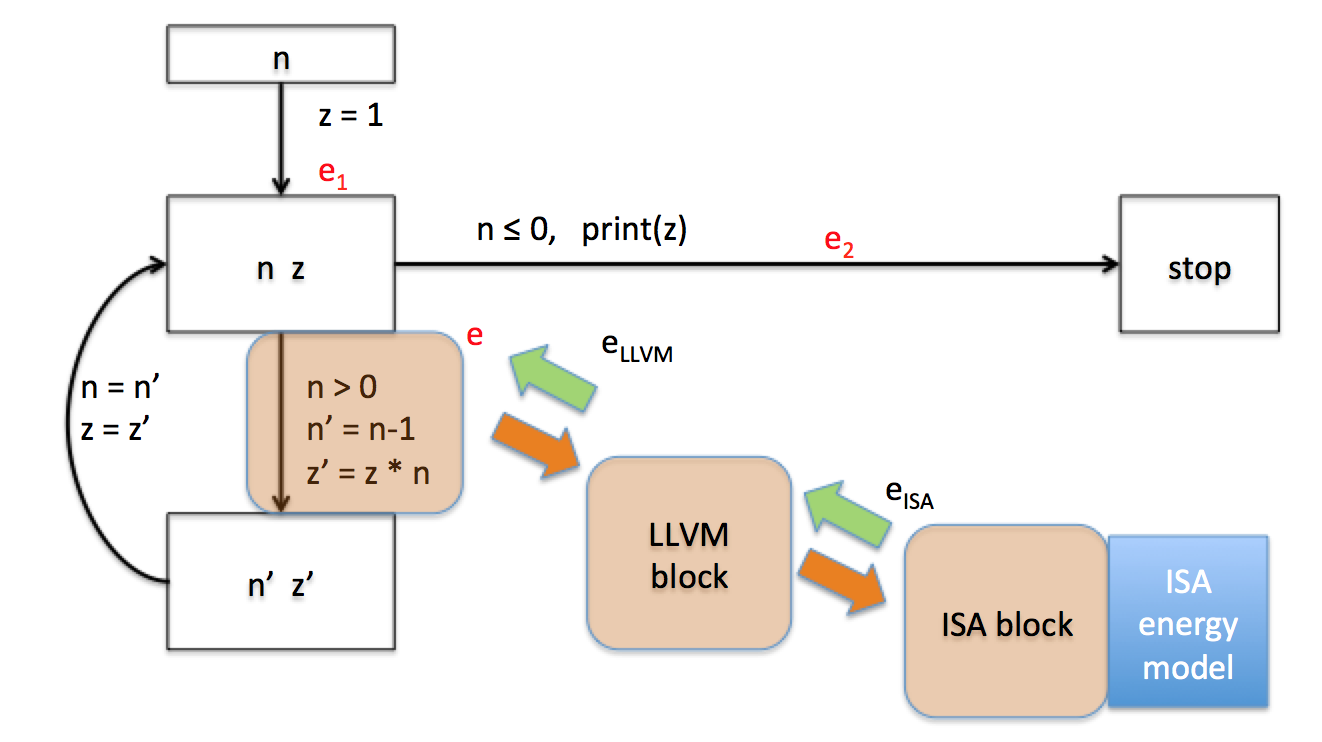
\includegraphics[width=8cm]{\figpath/mapping}   
 \caption{Combining an energy model with program analysis}
 \label{fig-model-mapping}
 \end{figure}

\subsection{Semantic representations of programs}
Static analysis of a program, and in general any formal treatment of programs, requires reference 
to a semantic model of the program derived from the semantics of the
programming language in which it is written. Several different semantic styles
and notations are used, including denotational semantic, small-step or structured
operational semantics, and big-step or natural operational semantics.
All of these can be applied to code
 at various levels such as source code, intermediate compiler
representations or ISA.

A common representation language, suitable mainly for operational semantics, is
constrained Horn clauses (CHCs), a subset of first order logic which is
widely used in software verification
\cite{DBLP:conf/birthday/BjornerGMR15}. CHCs can represent code semantics at any
level of abstraction. In this section we outline the key aspects of
resource analysis using CHCs as a representation, but space does not
allow a fully detailed presentation.  More information can be found in the
references given in the text.

A constrained Horn clause has the form $\forall x_0 \ldots x_n 
(p_1(x_1) \wedge \ldots \wedge p_n(x_N) \wedge \phi \rightarrow
p_0(x_0))$. When representing program semantics, each predicate
$p_0,p_1,\ldots,p_n$ typically corresponds to a program point, and its
respective arguments $x_0,x_1,\ldots,x_n$ are tuples representing the
state before and/or after those points.  A clause thus represents a
relationship between program states, and the constraint $\phi$ expresses
the relationship between the values of the state variables. A special case
of a Horn clause is where $n \le 1$, that is, there is at most one atomic
formula on the left of the clause.  Such a clause often represents a transition 
from the state at one program point to the next.

Figure \ref{fig-horn} illustrates the use of Horn clauses to 
represent an imperative program in a C-like language (a).
The constrained Horn clauses (b) represent a transition
system (c) induced by the program's small-step operational 
semantics (the quantifiers in
the Horn clauses are
omitted).  The predicates
$r_1, \ldots, r_4$ represent the program points $1,\ldots,4$ and
$r_i(x_i)$ means that program point $i$  is reachable with state
$x_i$, where $x_i$ is the tuple of variables in scope at that point.

Lower-level programs such as ISA or intermediate code can be translated
in a similar fashion, where typically each predicate represents a basic block 
in the code. Examples of the translation of XCore ISA programs
to Horn clauses are given in \cite{isa-energy-lopstr13-final}.
Semantics-based methods for translating sequential
imperative programs to
Horn clauses are explained in \cite{DBLP:conf/ppdp/AngelisFPP15}.
Furthermore techniques for representing multi-threaded
code as Horn clauses have been developed \cite{ GrebenshchikovLPR12}.


\subsection{Techniques for energy analysis}

Given such a representation of a program, techniques based on abstract interpretation \cite{Cousot1977}
can derive safe approximations of program behaviour.
In terms of CHCs, abstract interpretation can yield
safe approximations of the values of the arguments of each predicate, which represents the
set of possible
states at some program point.
A branch of abstract interpretation 
focusses on automatic complexity analysis, yielding complexity functions on the
execution time of the program \cite{DBLP:journals/cacm/Wegbreit75,Rosendahl89,caslog,resource-iclp07,jvm-cost-esop}.  
These techniques have been widely applied to
analysis of Horn clauses, and have been extended to analysis of energy and
other resources \cite{resource-iclp07,jvm-cost-esop}. Tools such as CiaoPP \cite{ciaopp-sas03-journal-scp} 
and COSTA \cite{AlbertAGPZ08b} have inbuilt
facilities for resource analysis of programs including CHCs.

The essence of the techniques is to extract constraints from the Horn clauses
representing the energy consumed. These constraints represent an abstraction of the behaviour
of the program, in which the energy (or other resource being considered)
can be considered as an implicit extra argument in the predicates of the Horn clauses.
(In some approaches, the extra resource arguments are actually inserted into
the Horn clauses, yielding a so-called ``instrumented" representation).
These constraints are then solved, or approximated, to yield explicit 
formulas giving the consumption.


 
\paragraph{Linking analysis to an energy model.} The Horn clauses in the semantic
representation can be 
associated with energy values, using an energy model. For example, if the clauses are obtained
from the source code, then each clause represents the execution of one statement or
source code expression, and a corresponding source code energy model is associated with
that clause.
If the clauses are obtained from lower-level code such as ISA, a clause typically represents 
the execution of
an instruction or basic block;  the corresponding energy consumption from the model can be
mapped to the clause. The energy from a lower-level model
such as an ISA model can also be mapped to a Horn clause representing 
a higher-level construct, possibly via an intermediate level as indicated in Figure \ref{fig-model-mapping}. 

Once this is done, constraints
representing the energy consumption of the program are extracted from the Horn clause 
representation. To make the explanation more intuitive, we explain the process in terms of the transition system,
rather than the Horn clause representation. In the case of the loop at point 2, a recursive equation is obtained, e.g.
\[ cost_2(n) = e + cost_2(n-1)~ (\mathrm{if}~n > 0), ~~cost_2(n) = 0 ~ (\mathrm{if}~n \le 0) \]
where $e$ is the energy cost of one iteration of the loop, obtained from the energy model. A dependency analysis
also determines that the variable $n$ is the relevant input parameter in this case. These
equations can be solved to yield the expression giving the cost of the loop as a function of $n$, 
namely $cost_2(n) = n*e$, and the cost of the whole 
program (a path from 1 to 4) is $cost(n) = e_1 + n*e + e_2$, where $e_1, e_2$ are the respective
energy costs of the transitions before and after the loop.

\paragraph{More complex analyses.} The example shown is very simple, but the method generalises to
more complex control and data structures.  
As the data and control-flow analysis of abstract interpretation is inherently approximate, 
the analysis in general gives safe upper and lower bounds on the 
number of times each part of the program is executed. This in turn gives upper and lower bounds on the energy
consumed by the program.  However, recall that the upper and lower bounds are also relative to the energy model,
as discussed in Section \ref{subsec:data}. If the energy model supplies average costs for the basic instructions
or operations, then the upper and lower bounds on the energy given by the analysis might not be safe, since the
actual costs of executing the instructions might be respectively higher or lower than the average.

A further extension of the method of generating constraints and solving them yields
static energy profiling~\cite{staticprofiling-flops}, which shows the
distribution of energy usage over the parts of the code, rather than a single function giving the total consumption of the program.
